\def\iangle{35} % Angle of the inclined plane
\def\down{0}
\def\arcr{0.7cm} % Radius of the arc used to indicate angles
\newcommand\centerofmass{%
    \tikz[radius=0.2em] {%
        \fill (0,0) -- ++(0.2em,0) arc [start angle=0,end angle=90] -- ++(0,-0.4em) arc [start angle=270, end angle=180];%
        \draw (0,0) circle;%
    }%
}

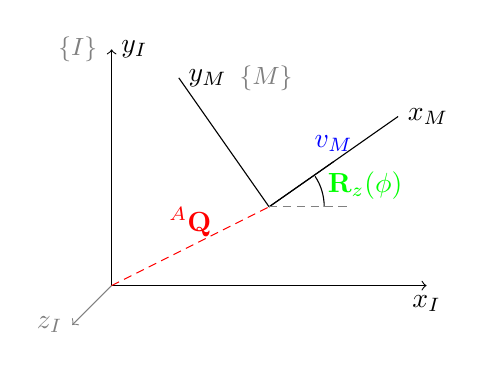
\begin{tikzpicture}[
    force/.style={>=latex,draw=blue,fill=blue},
    axis/.style={densely dashed,gray,font=\small},
    M/.style={rectangle,draw,fill=lightgray,minimum size=0.7cm,thin},
    m/.style={rectangle,draw=black,fill=lightgray,minimum size=0.3cm,thin},
    plane/.style={draw=black,fill=blue!10},
    string/.style={draw=red, thick},
    pulley/.style={thick},
    wheel/.style={fill=black, rounded corners=1.5pt},
]
    %% Free body diagram of M
    \begin{scope}[rotate=\iangle]
        \node[] (M) {};
%        \node[below, purple] at (M) {${}^B_A\mathbf{P}$};
        % Draw axes and help lines
        {[axis,->]
            \draw (M.center) -- ++(0,2) node(y1_axis)[right] {$y_M$};
            \draw (M.center) -- ++(2,0) node[right] {$x_M$};
            % Indicate angle. The code is a bit awkward.
            \draw[solid,shorten >=0.5pt] (\down-\iangle:\arcr)
                arc(\down-\iangle:\down:\arcr);
            \node[xshift=10, green]at (\down-0.5*\iangle:1.3*\arcr) {$\mathbf{R}_z(\phi)$};
        }
        % Forces
        {[force,->]
            % Assuming that Mg = 1. The normal force will therefore be cos(alpha)
            \draw (M.center) -- ++(1,0) node[above, blue] {$v_M$};
        }
    \end{scope}
    % Draw gravity force. The code is put outside the rotated
    % scope for simplicity. No need to do any angle calculations. 
    \draw[axis,] (M.center) -- ++(1,0) node[below] {};
    %%
    \node[right, gray,font=\small, xshift=8] at (y1_axis) {$\{M\}$};
    %%
    \draw[, ->] (-2,-1) -- ++(4,0) node[below] {$x_I$};
    \draw[, ->] (-2,-1) -- ++(0,3) node(y_axis)[right] {$y_I$};
    \draw[gray, ->] (-2,-1) -- ++(-.5,-.5) node[left] {$z_I$};
    \node[left, gray,font=\small, xshift=-10] at (y_axis) {$\{I\}$};
    \draw [densely dashed,red,] (-2,-1)-- (M.center) node[above, midway] {${}^A\mathbf{Q}$};
\end{tikzpicture}

  